\documentclass{beamer}
\usepackage[T1]{fontenc}
\usepackage[utf8]{inputenc}
\usepackage{graphicx}
\usepackage[normalem]{ulem}
\usepackage{xmpmulti}
% \usepackage[dvipsnames]{xcolor}
% \usepackage{enumitem}


\newcommand{\emphh}[1]{\textcolor{blue}{\emph{#1}}}
\newcommand{\hilite}[1]{\emphh{#1}}
\title{Erdős-Pósa for Pairwise Distant Cycles}

\newcommand{\verteq}{\rotatebox{90}{$\equiv$}}

\author{}
\author{%
  Vida~Dujmović \and
  Gwenaël~Joret \and
  Piotr~Micek \and
  Pat Morin \\[3ex]
  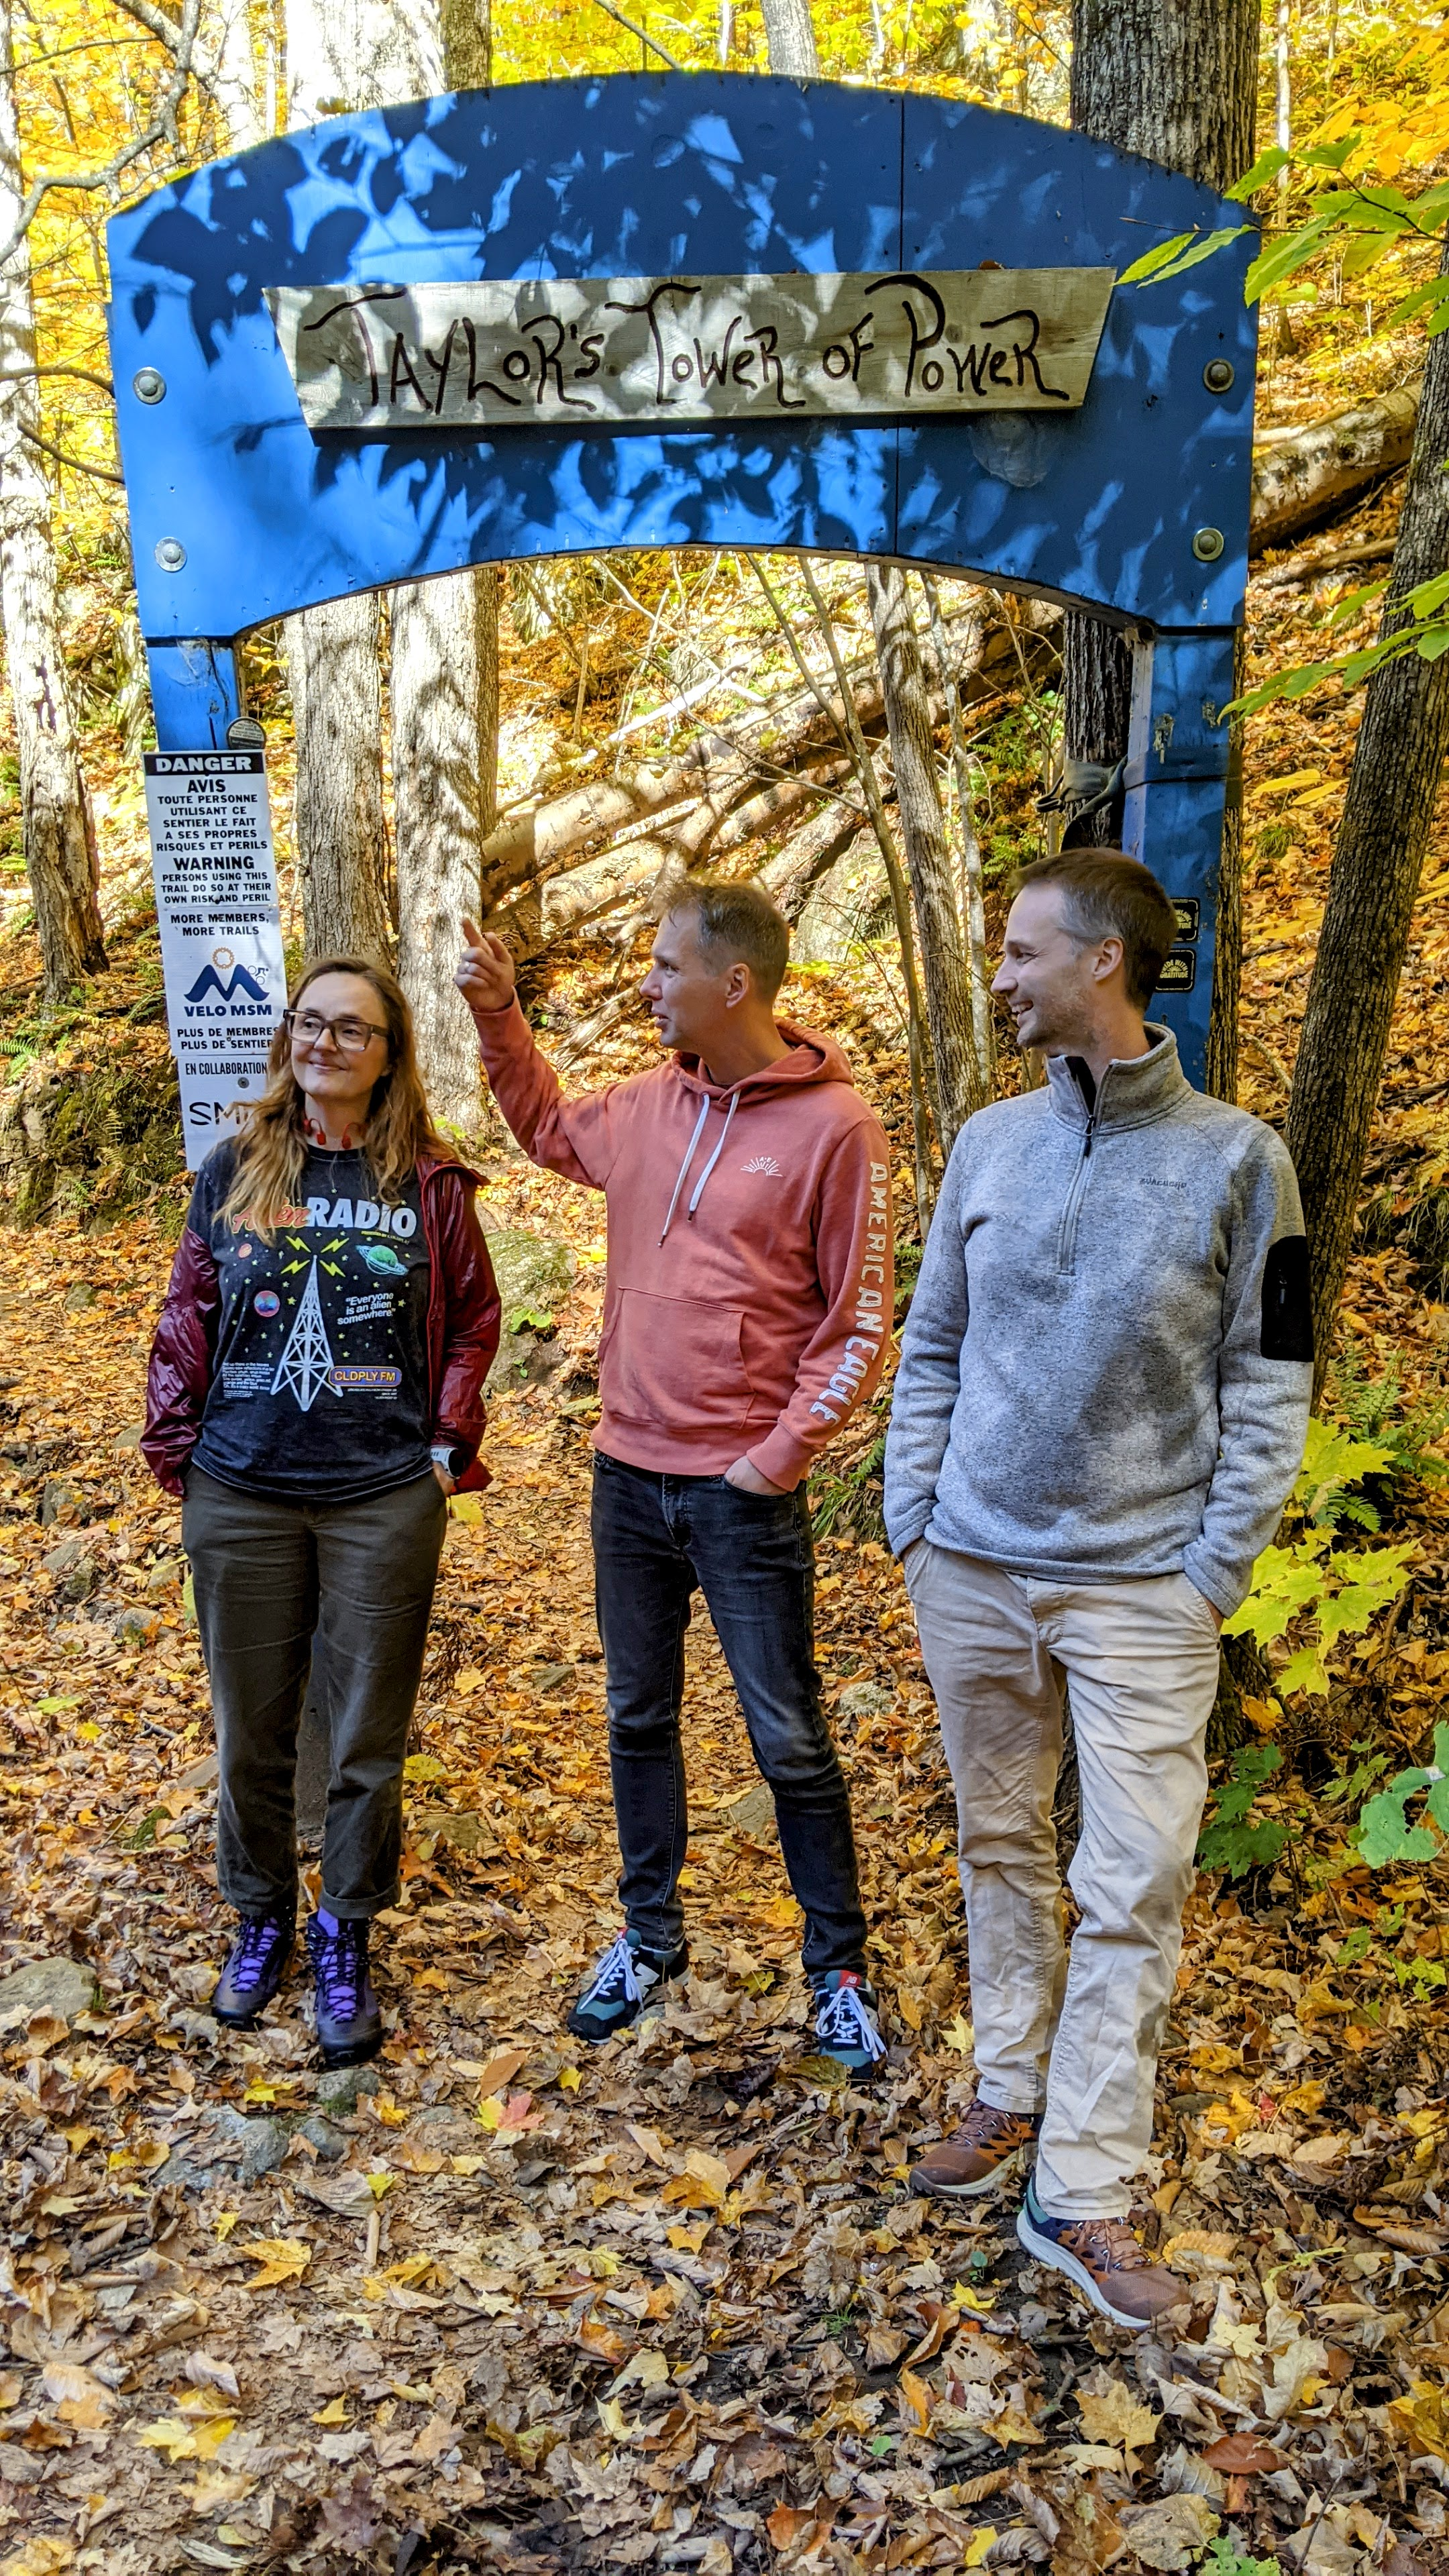
\includegraphics[height=.4\textheight]{images/ttop-hdr}
  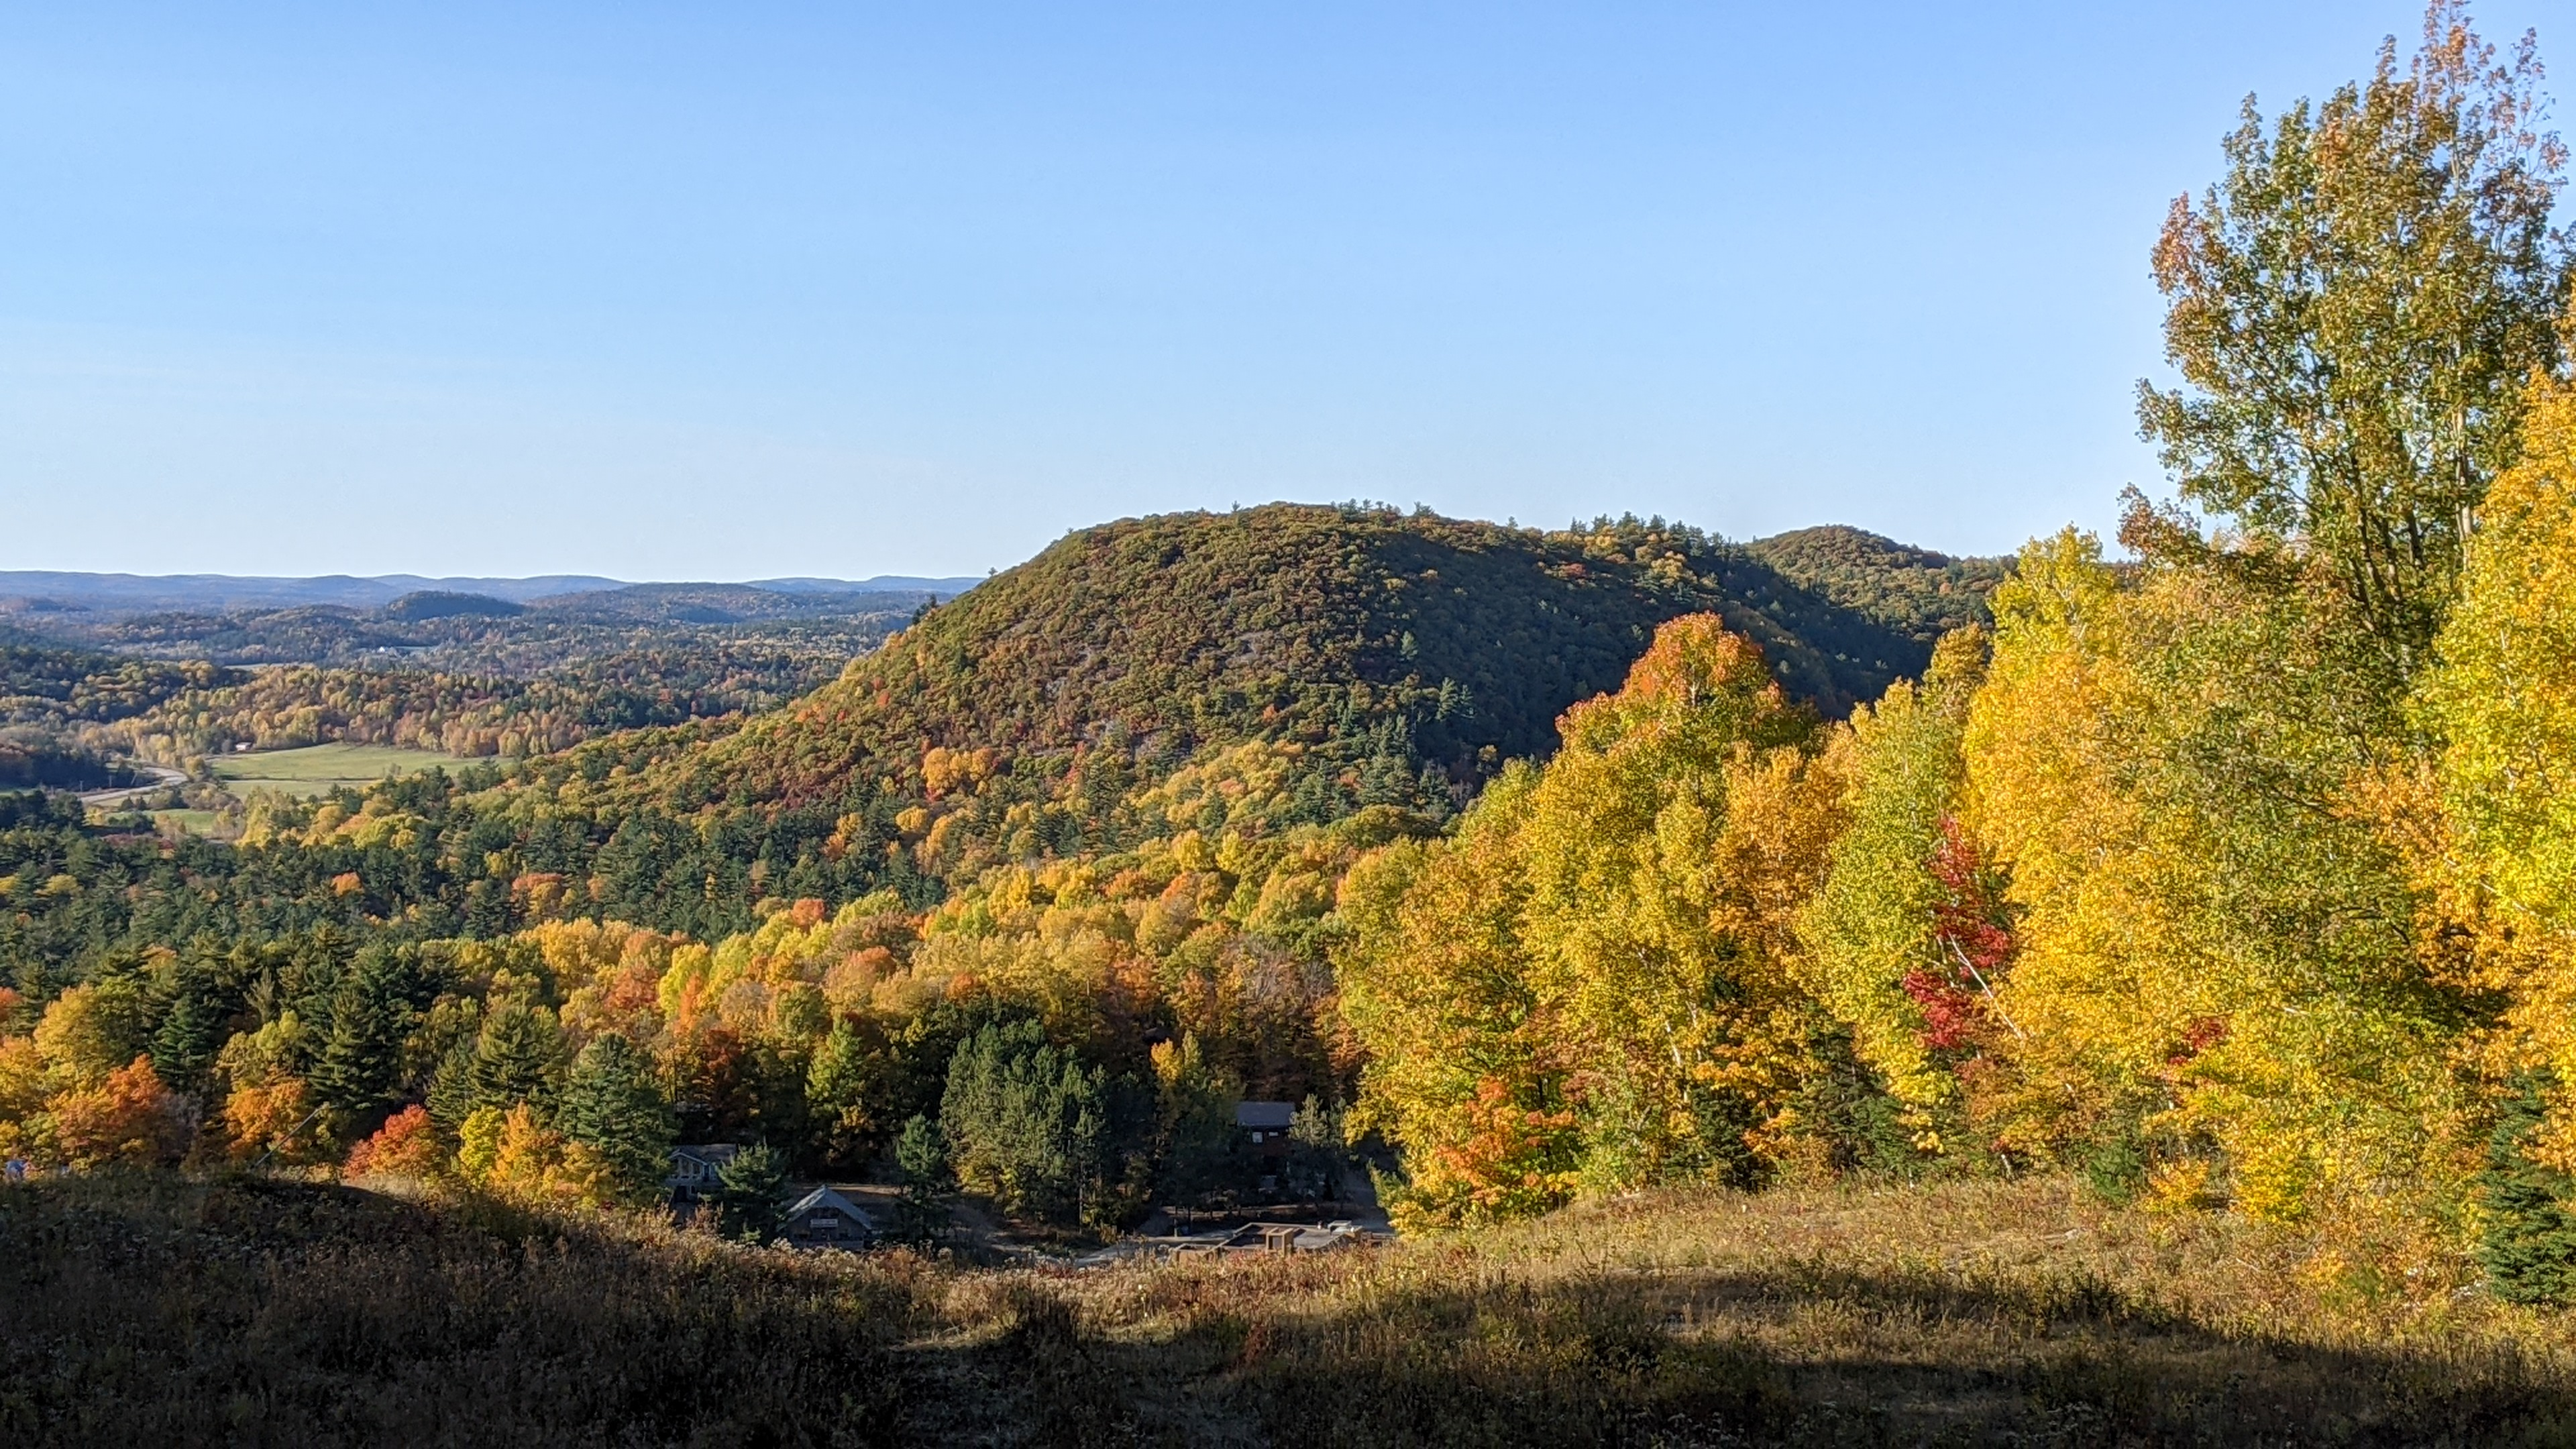
\includegraphics[height=.4\textheight]{images/view}}
\date{}

\setbeameroption{hide notes} % Only slides
%\setbeameroption{show only notes} % Only notes
% \setbeameroption{show notes on second screen=right} % Both


% \DeclareMathOperator{\tw}{tw}
% \DeclareMathOperator{\td}{td}
% \DeclareMathOperator{\wcol}{wcol}
% \DeclareMathOperator{\lvr}{\chi_{\ell-\mathrm{vr}}}
% \DeclareMathOperator{\pcn}{\chi_{p}}

\begin{document}

\begin{frame}
  % \begin{center}
    \maketitle
  % \end{center}
\end{frame}

\begin{frame}
  \frametitle{Outline}

  \begin{itemize}
    \item Theorem statement
    \item Some related work
    \item Proof sketch
  \end{itemize}
\end{frame}


\begin{frame}
  \frametitle{Main Theorem}

  \noindent\textbf{Theorem (Dujmović-Joret-Micek-M 2024):} For every graph $G$, every integer $k\ge 1$ and $d\ge 0$,
  \begin{enumerate}%[nosep,nolistsep]
    \item $G$ contains \textcolor{blue}{$d$-packing} of $k$ cycles \textbf{or}
    \item $G$ has a vertex subset $\mathcolor{red}{X}$ of size at most $f(k)$ such that $G-B_G(X,g(d))$ is a forest.  \newline \uncover<2->{(Every cycle in $G$ contains a vertex in $\mathcolor{blue}{B_G(X, g(d))}$.)}
  \end{enumerate}

  \begin{center}
    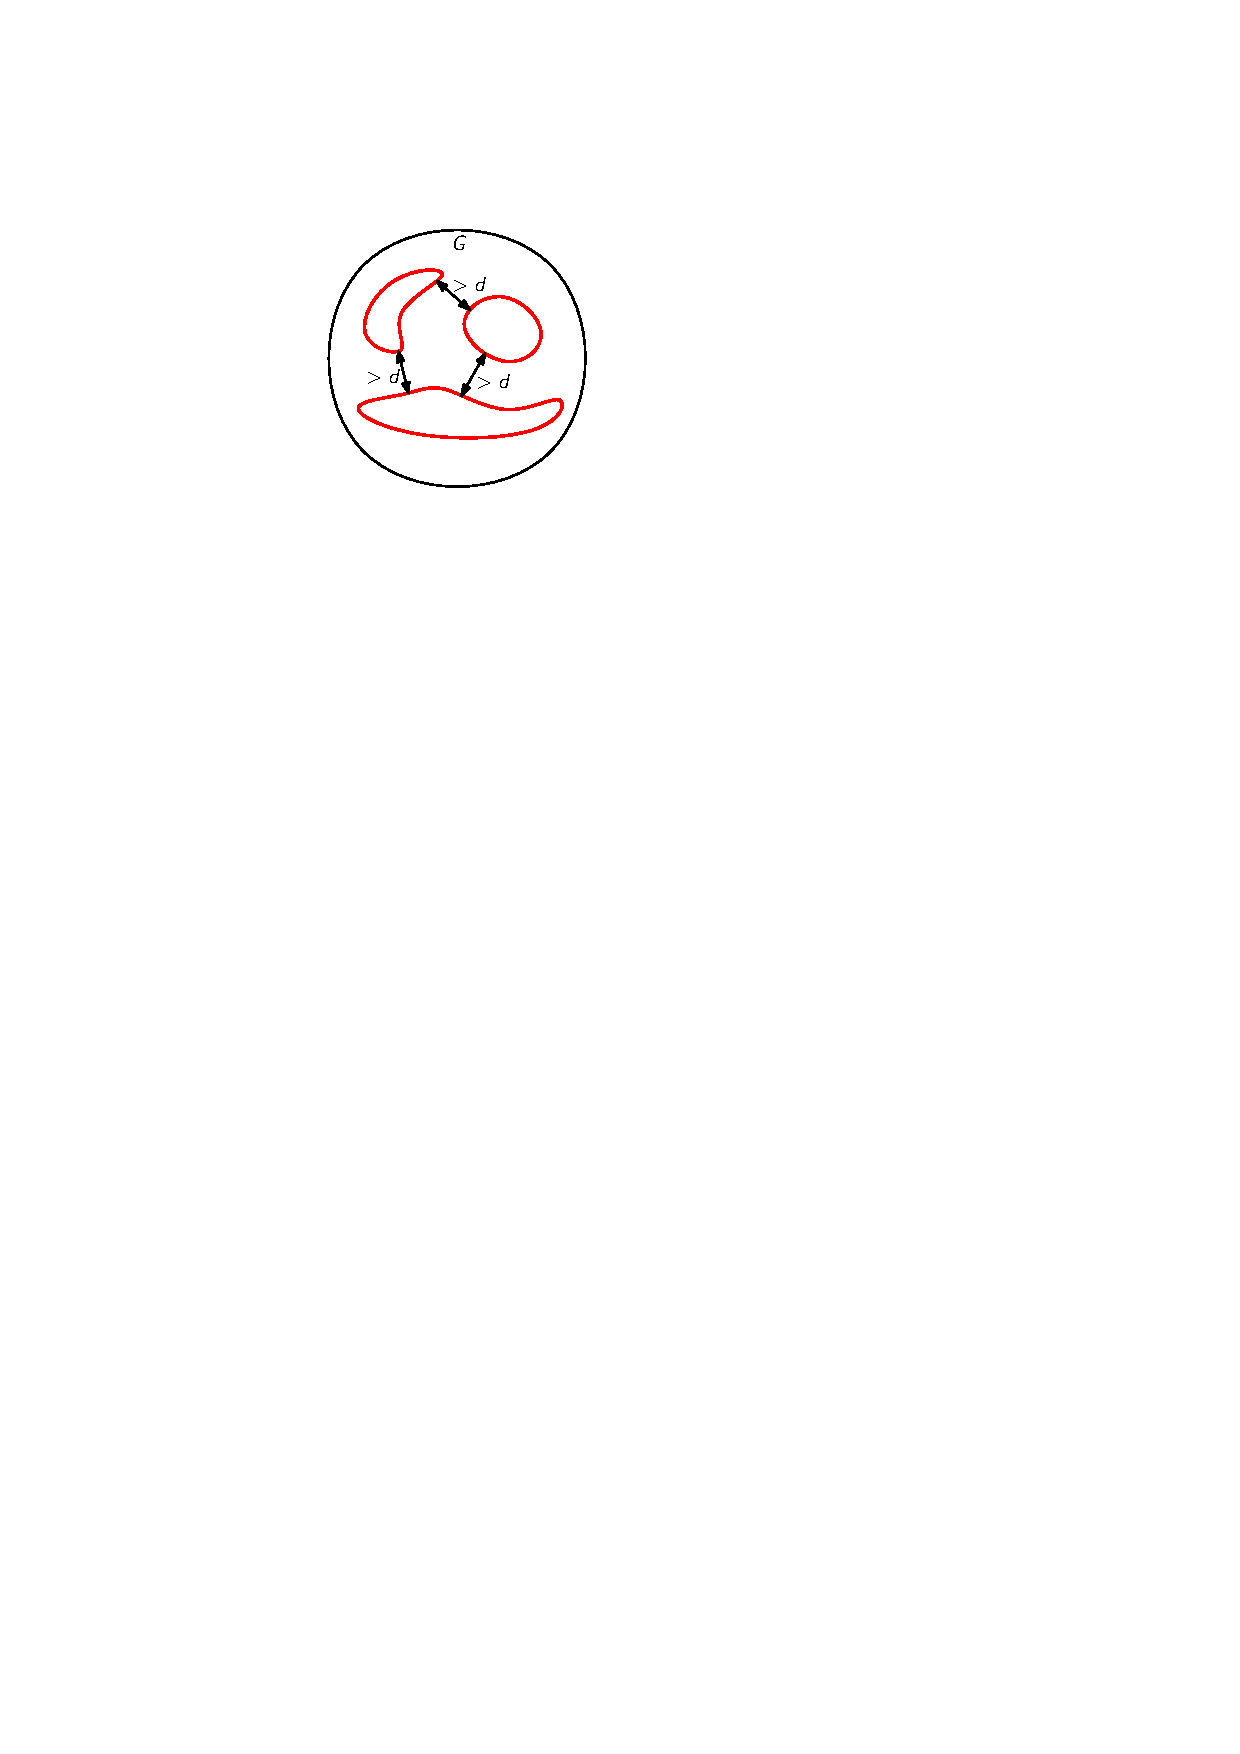
\includegraphics[scale=.9,page=1]{figs/cep}
    \raisebox{2cm}{ OR }
    \includegraphics[scale=.9,page=2]{figs/cep}
  \end{center}
  \uncover<3->{(And $f(k)\in O((k\log k)^{18})$ and $g(d)\le 19d$.)}
\end{frame}


\begin{frame}
  \frametitle{The Erdős-Pósa Theorem}

    \noindent\textbf{Theorem (Erdős-Pósa 1965):}
    For every graph $G$ and every integer $k\ge 1$,
    \begin{enumerate}%[nosep,nolistsep]
      \item $G$ contains $k$ pairwise vertex-disjoint cycles \textbf{or}
      \item $G$ has a vertex subset $\mathcolor{red}{X}$ of size $O(k\log k)$ such that $G-X$ is a forest. \uncover<3>{\textcolor{blue}{(Every cycle in $G$ has a vertex in $X$.)}}
    \end{enumerate}
    \begin{center}
      \only<1>{\includegraphics[page=3]{figs/erdos_posa}}%
      \only<2->{\includegraphics[page=4]{figs/erdos_posa}}
      \uncover<2->{\raisebox{2cm}{ OR }}
      \only<1>{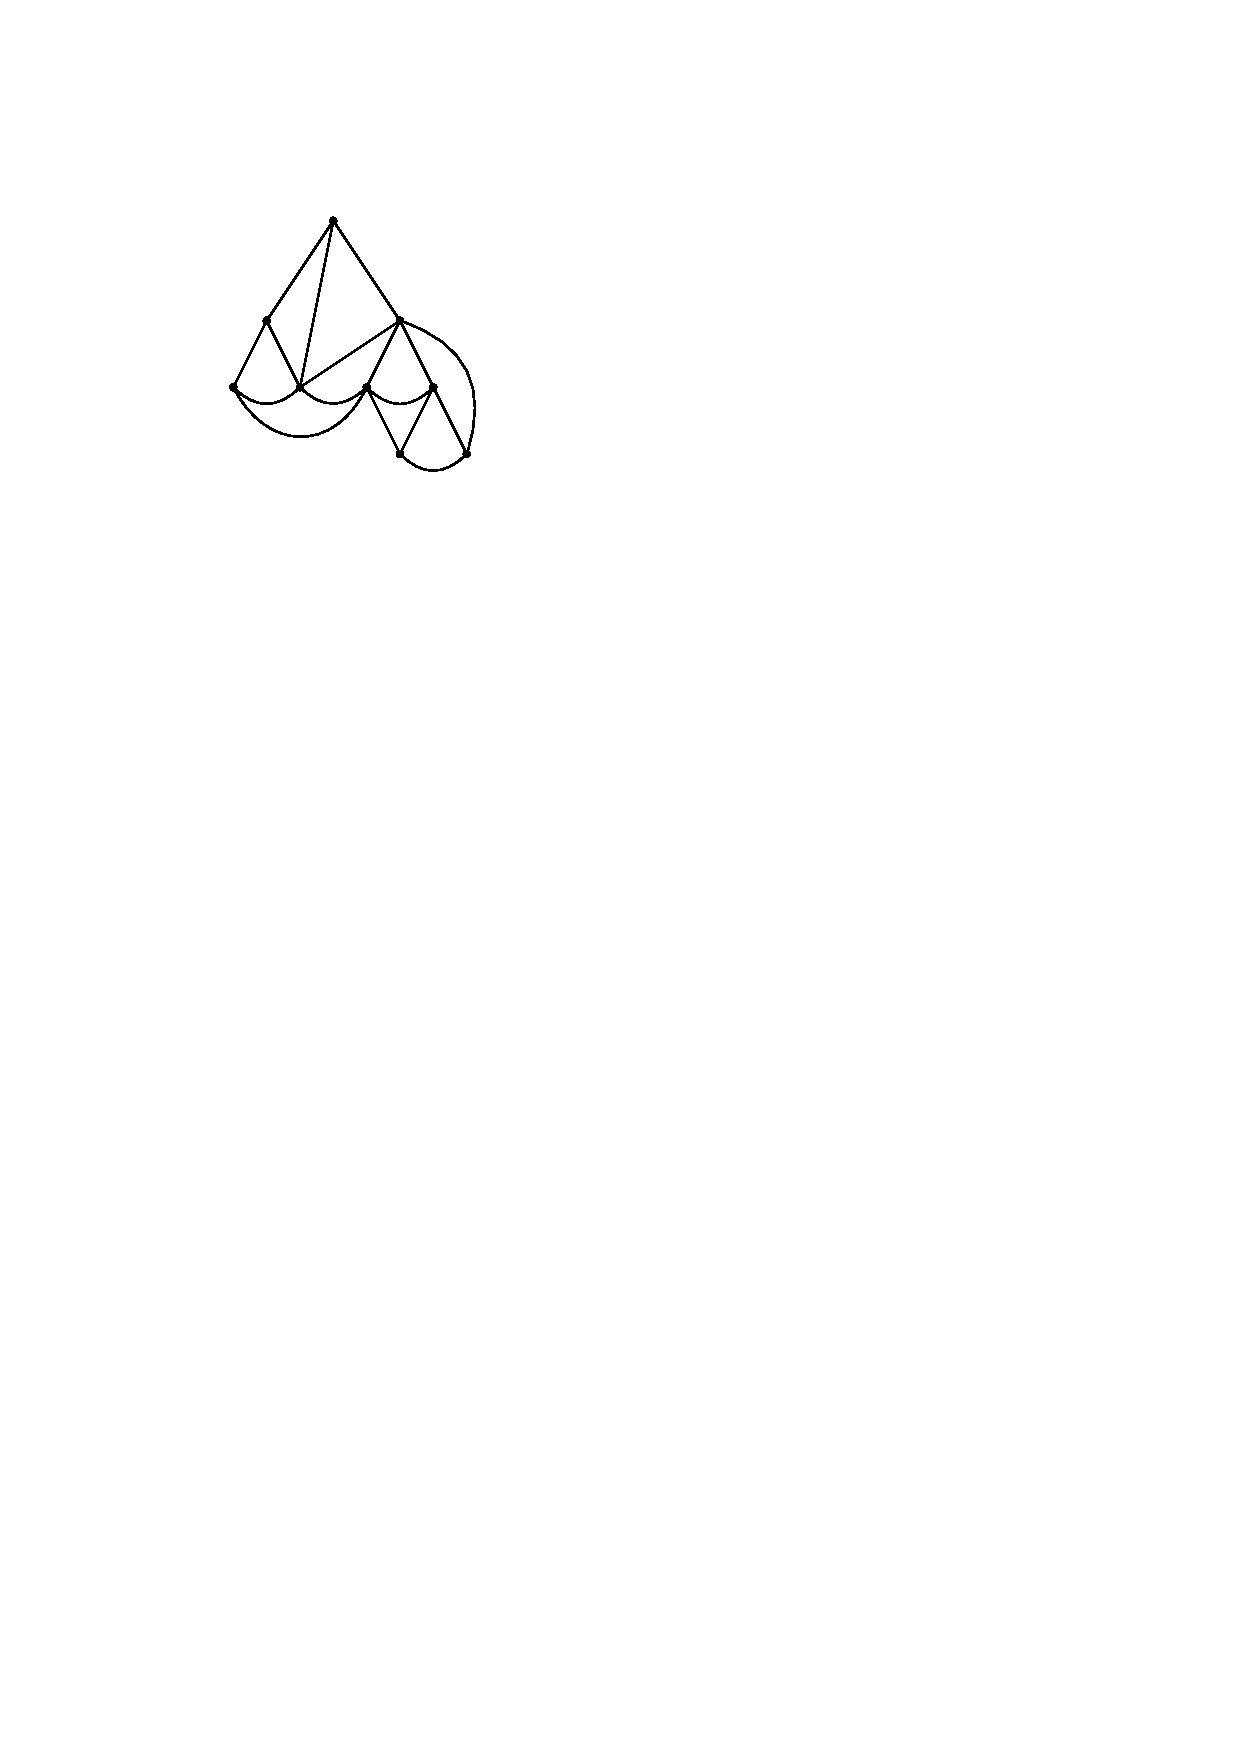
\includegraphics[page=1]{figs/erdos_posa}}%
      \only<2->{\includegraphics[page=2]{figs/erdos_posa}}
    \end{center}
\end{frame}


\begin{frame}
  \frametitle{A Robertson-Seymour Erdős-Pósa-Type Theorem}

  \noindent\textbf{Theorem (Robertson-Seymour 1986):} For every graph $G$, every integer $k\ge 1$,  and every planar graph $H$,
  \begin{enumerate}%[nosep,nolistsep]
    \item $G$ contains $k$ pairwise vertex-disjoint $H$ minors \textbf{or}
    \item $G$ has a vertex subset $\mathcolor{red}{X}$ of size at most $f(H)$ such that $G-X$ is $H$-minor-free. \textcolor{blue}{(Every model of $H$-minor of $G$ has a vertex in $X$.)}
  \end{enumerate}
\end{frame}


\begin{frame}
  \frametitle{An Erdős-Pósa-Type Theorem for Subtrees}

  \noindent\textbf{Theorem:} For every tree $T$, every integer $k\ge 1$,  and every collection $\mathcal{C}$ of subtrees of $T$,
  \begin{enumerate}%[nosep,nolistsep]
    \item $\mathcal{C}$ contains $k$ pairwise vertex-disjoint subtrees \textbf{or}
    \item $G$ has a vertex subset $\mathcolor{red}{X}$ of size at most $k-1$ such that every subtree in $\mathcal{C}$ contains a vertex in $X$.
  \end{enumerate}
\end{frame}


\begin{frame}
  \frametitle{An Erdős-Pósa-Type Theorem for $c$-Subtrees}

  \noindent{\textbf{Definition:} A $c$-forest in a forest $F$ is a subgraph of $F$ with at most $c$ components.\\[3ex]}

  \noindent\textbf{Theorem (Gyárfás-Lehel 1970):} For every forest $F$, every integer $k\ge 1$, and every collection $\mathcal{C}$ of $c$-subtrees of $F$,
  \begin{enumerate}%[nosep,nolistsep]
    \item $\mathcal{C}$ contains $k$ pairwise vertex-disjoint $c$-subtrees \textbf{or}
    \item $G$ has a vertex subset $\mathcolor{red}{X}$ of size at most $\ell^\star(k,c)$ such that every $c$-subtree in $\mathcal{C}$ contains a vertex in $X$.
  \end{enumerate}
\end{frame}


\begin{frame}
  \frametitle{Simonovits' Theorem}


  \noindent\textbf{Theorem (Simonovits 1967):} Every cubic graph $G$ with at least $C k\log k$ vertices contains $k$ pairwise vertex-disjoint cycles.
\end{frame}


\begin{frame}
  \frametitle{An Erdős-Pósa-Type Theorem for Pairwise-Distant Cycles}

  \noindent\textbf{Theorem (Dujmović-Joret-Micek-M 2024):} For every graph $G$, every integer $k\ge 1$ and $d\ge 0$,
  \begin{enumerate}%[nosep,nolistsep]
    \item $G$ contains \textcolor{blue}{$d$-packing} of $k$ cycles \textbf{or}
    \item $G$ has a vertex subset $\mathcolor{red}{X}$ of size at most $f(k)$ such that every cycle in $G$ contains a vertex in $\mathcolor{blue}{B_G(X, g(d))}$.
  \end{enumerate}

  \begin{center}
    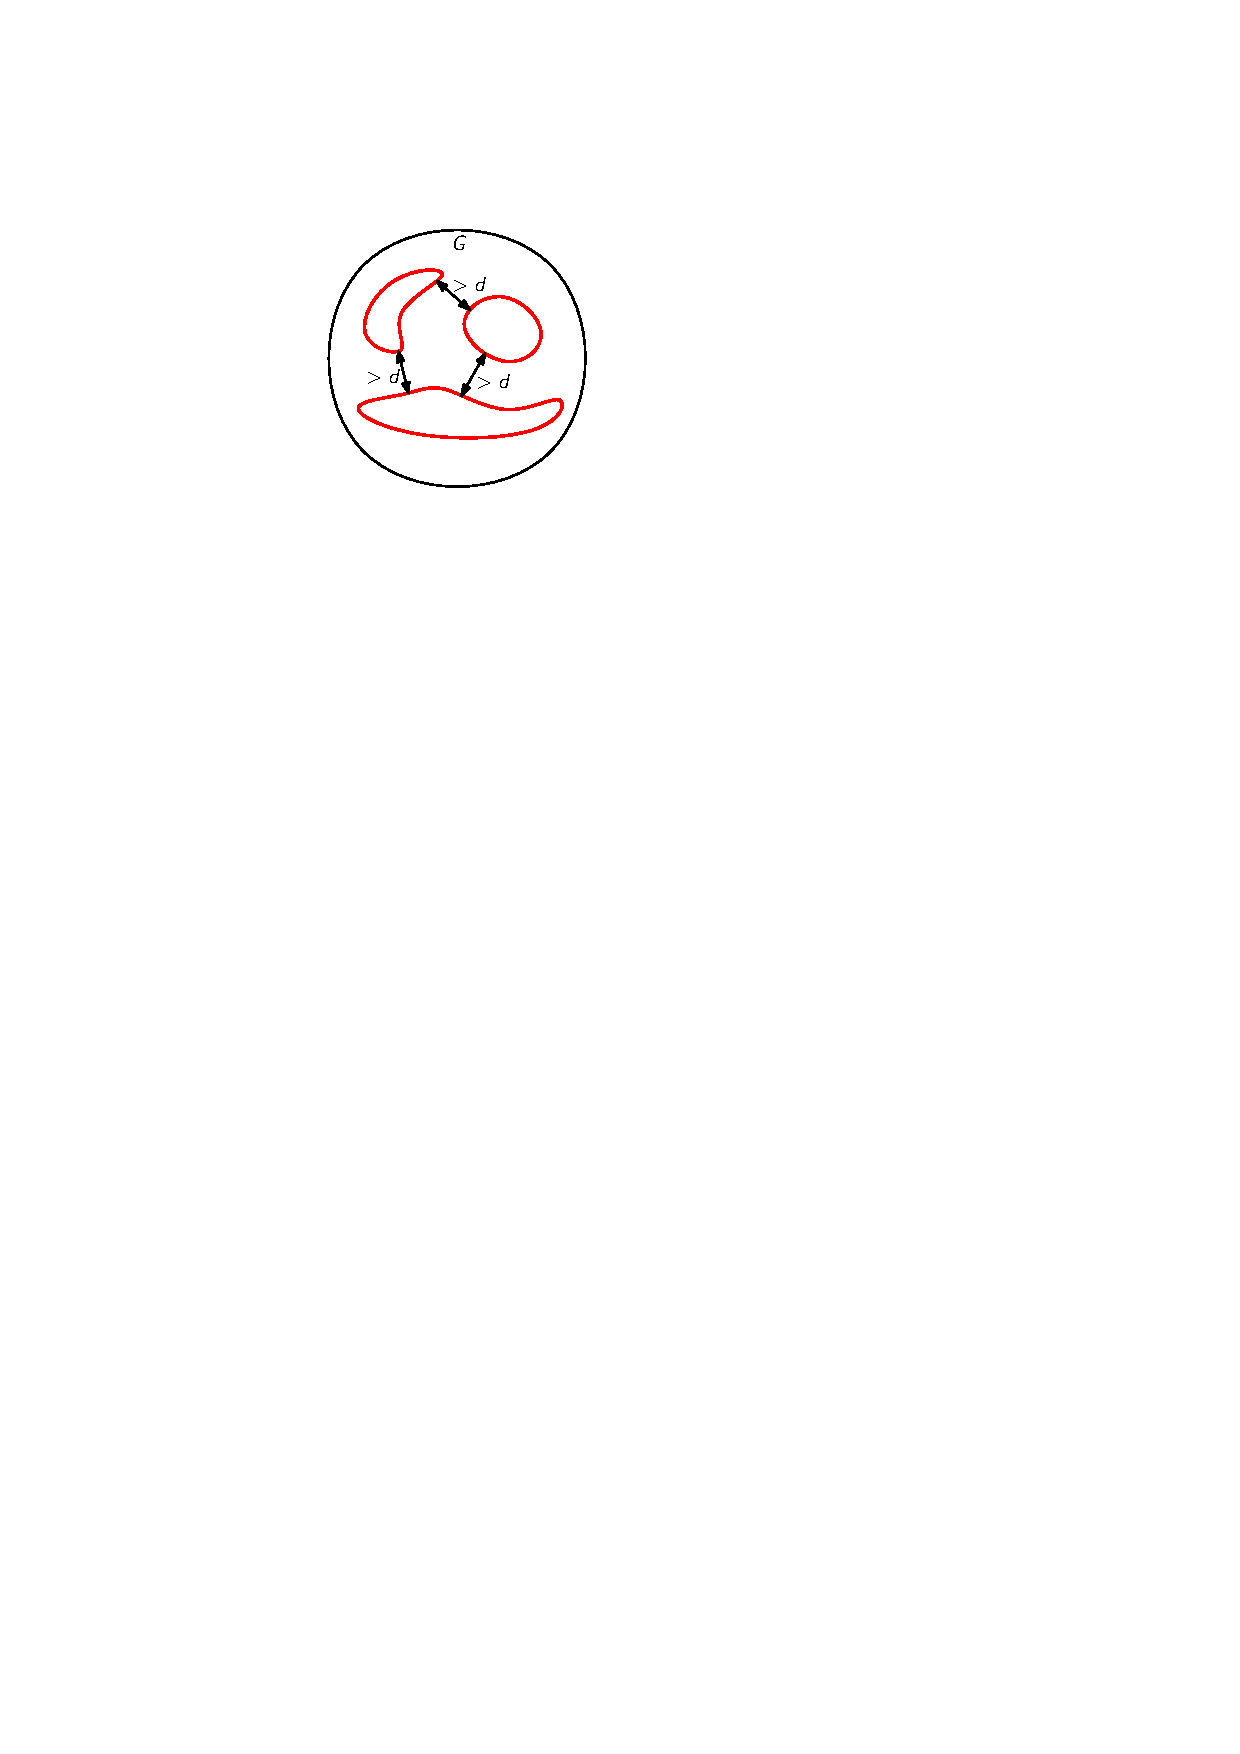
\includegraphics[page=1]{figs/cep}
    \raisebox{2cm}{ OR }
    \includegraphics[page=2]{figs/cep}
  \end{center}
\end{frame}

\begin{frame}
  \frametitle{Proof Outline}

  \only<1>{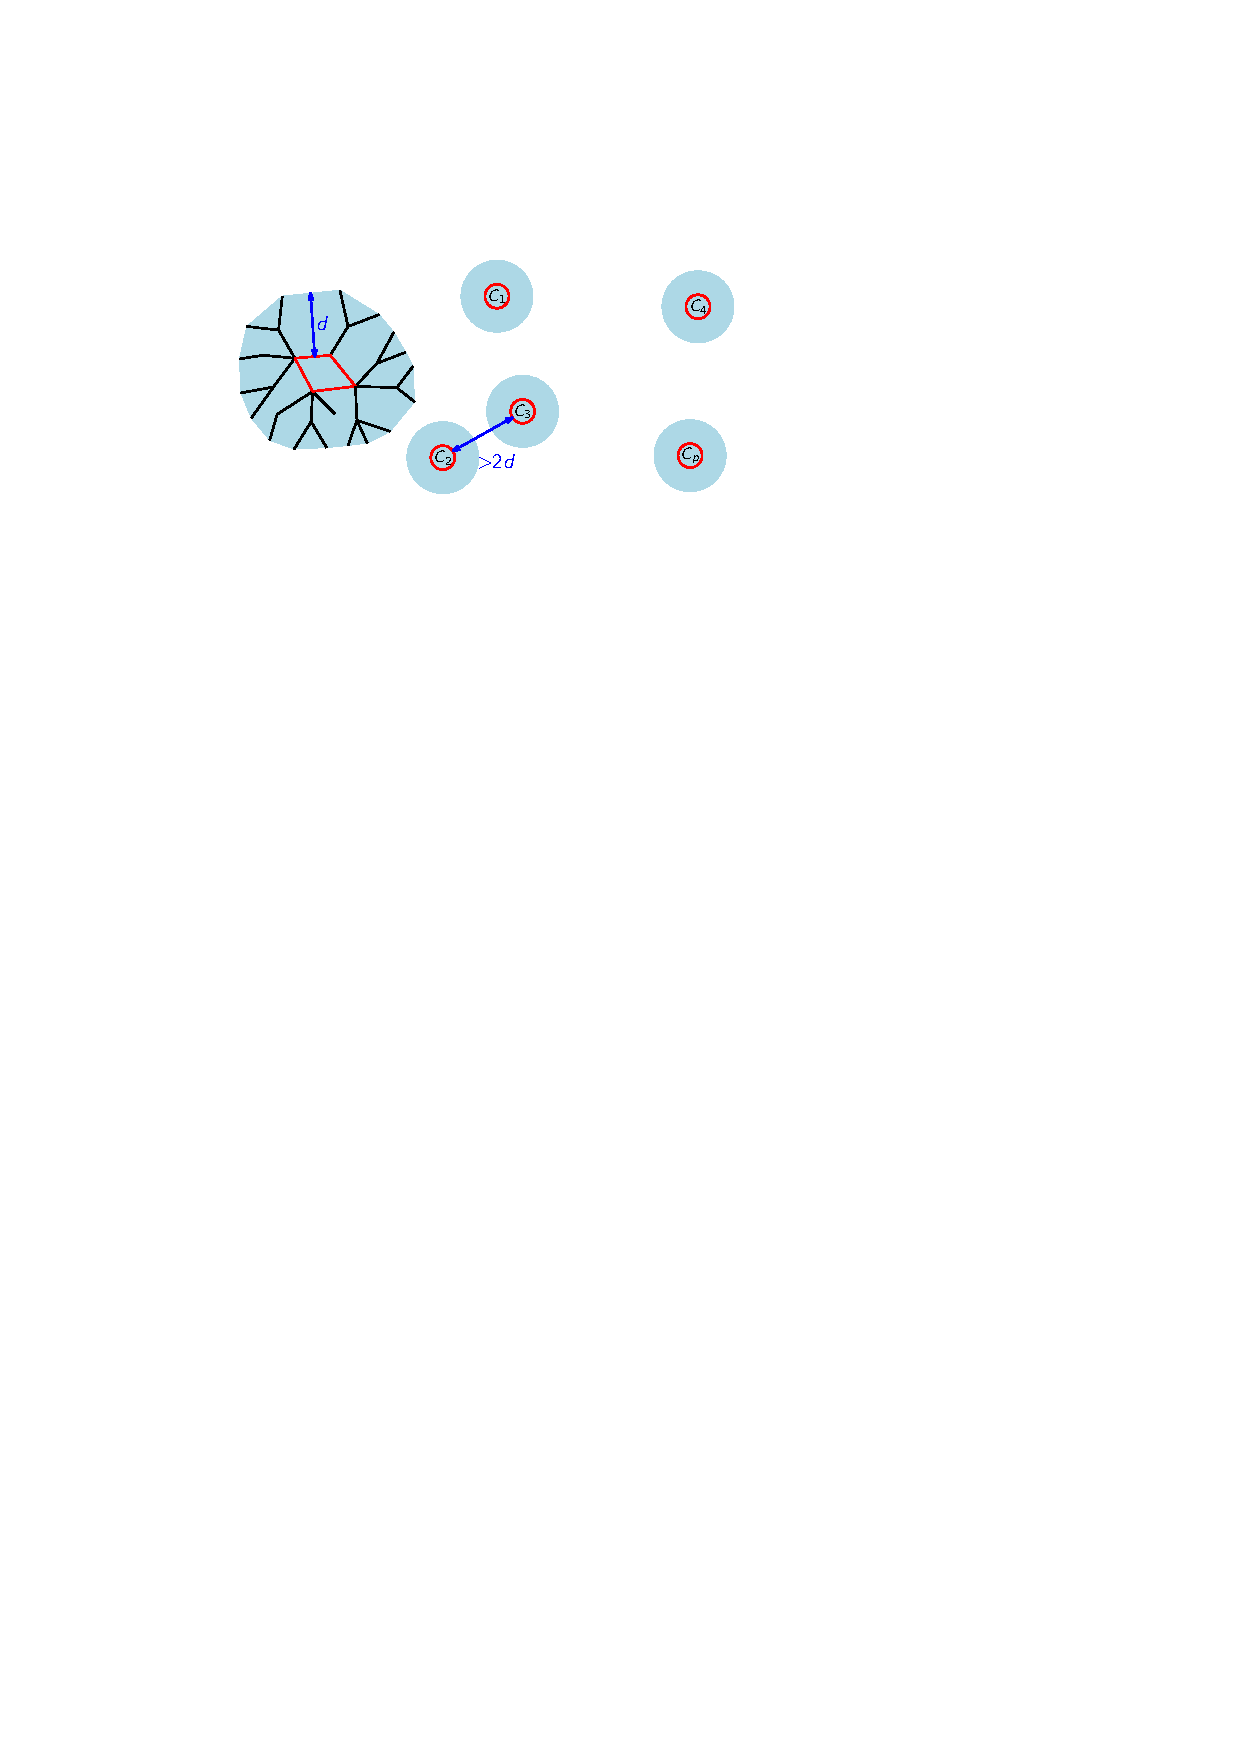
\includegraphics[page=1]{figs/animation}}%
  \only<2>{\includegraphics[page=2]{figs/animation}}%
  \only<3>{\includegraphics[page=3]{figs/animation}}%
  \only<4>{\includegraphics[page=4]{figs/animation}}%
  \only<5>{\includegraphics[page=5]{figs/animation}}%
  \only<6>{\includegraphics[page=6]{figs/animation}}%
  \only<7>{\includegraphics[page=7]{figs/animation}}%
  \only<8-9>{\includegraphics[page=8]{figs/animation}}%
  \only<10>{\includegraphics[page=9]{figs/animation}}%
  \only<11>{\includegraphics[page=10]{figs/animation}}%
  \only<12>{\includegraphics[page=11]{figs/animation}}%
  \only<13>{\includegraphics[page=12]{figs/animation}}%
  \only<14>{\includegraphics[page=13]{figs/animation}}%
  \only<15>{\includegraphics[page=14]{figs/animation}}%
  \only<16>{\includegraphics[page=15]{figs/animation}}%
  \only<17>{\includegraphics[page=16]{figs/animation}}%
  \only<18>{\includegraphics[page=17]{figs/animation}}%
  \only<19>{\includegraphics[page=18]{figs/animation}}%
  \only<20-21>{\includegraphics[page=19]{figs/animation}}%

  \only<1>{Start with maximal $2d$-packing $\mathcal{C}:=\{C_1,\ldots,C_p\}$ of $d$-unicyclic cycles}%
  \only<2>{\textbf{Lemma$^\star\colon$} Any cycle in $G$ is \textcolor{blue}{short} or \textcolor{blue}{close to} a cycle in $\mathcal{C}$}%
  \only<3>{Iteratively hit each short cycle with a single ball of radius $7d+1$}%
  \only<4>{Every (unhit) cycle in $G$ is \textcolor{blue}{close to} a cycle in $\mathcal{C}$}%
  \only<5-8>{\textbf{Lemma$^\star\colon$} For each $i\in\{1,\ldots,p\}$,  $B_G(C_i,6d)-B_G(X_i,13d)$ is acyclic, for some $X_i$ with $|X_i|\le f'(k)$}%
  \only<9>{$F_i:=B_G(C_i,6d)-B_G(X_i,13d)$ is a forest, for each $i\in\{1,\ldots,p\}$}
  \only<10-12>{$F_0:=G-(\mathcolor{red}{B_G(X,7d+1)}\cup \mathcolor{blue}{\bigcup_{i=1}^p B_G(C_i,4d)})$ is a forest}%
  \only<13-14>{\textbf{Lemma$^\star\colon$} For each distinct $i,j\in\{1,\ldots,p\}$, $B_G(C_i,6d)\cap B_G(C_j,6d)\subseteq B_G(X_{\{i,j\}},13d)$, for some $X_{\{i,j\}}$ with $|X_{\{i,j\}}|\le f'(k)$}
  \only<15>{$(\bigcup_{i=1}^p B_G(C_i,6d))-(\bigcup_i B_G(X_i,13d)\cup \bigcup_{i,j}(B_G(X_{\{i,j\}},13d))$ is a forest}
  \only<16-17>{Any remaining cycle contain a \textcolor{blue}{segment} $s$ with parts in $F_0$, $F_i$, and $F_j$}%
  \only<18>{Segment $s$ has three parts $s_0$, $s_i$, $s_j$}%
  \only<19>{Extend $s_0$, $s_i$, and $s_j$}%
  \only<20>{$B_G(s_0,d)\subseteq F_0$, $B_G(s_i,d)\subseteq F_i$, and $B_G(s_j,d)\subseteq F_j$}%
  \only<21>{Map each segment to a $3$-subtree in a forest}

\end{frame}


\begin{frame}
  \frametitle{An Erdős-Pósa-Type Theorem for $c$-Subtrees}

  Recall:

  \noindent\textbf{Theorem (Gyárfás-Lehel 1970):} For every forest $F$, every integer $k'\ge 1$, and every collection $\mathcal{C}$ of $c$-subtrees of $F$,
  \begin{enumerate}%[nosep,nolistsep]
    \item $\mathcal{C}$ contains $k'$ pairwise vertex-disjoint $c$-subtrees \textbf{or}
    \item $G$ has a vertex subset $\mathcolor{red}{X}$ of size at most $\ell^\star(k',c)$ such that every $c$-subtree in $\mathcal{C}$ contains a vertex in $X$.
  \end{enumerate}
  \vspace{3ex}
  \uncover<2->{In Case~2, $B_G(X,4d)$ hits every remaining cycle in $G$}
  \vspace{2ex}
\end{frame}

\begin{frame}
  \frametitle{An Erdős-Pósa-Type Theorem for $c$-Subtrees}

  In Case 1:\\
  \only<1>{\includegraphics[page=19]{figs/animation}}%
  \only<2>{\includegraphics[page=20]{figs/animation}}

  \uncover<2->{Recall:\\
  \noindent\textbf{Theorem (Simonovits 1967):} Every cubic graph $G$ with at least $C k\log k$ vertices contains $k$ pairwise vertex-disjoint cycles.
  }
\end{frame}



\end{document}
